\scnheader{Реализация sc-хранилища и средств доступа к нему}
\scnrelfromlist{компонент программной системы}{Реализация sc-хранилища;Реализация файловой памяти ostis-системы}

\scnheader{Реализация sc-хранилища}
\scniselement{реализация sc-хранилища на основе линейной памяти}
\scnrelfrom{иллюстрация}{\scnfileimage{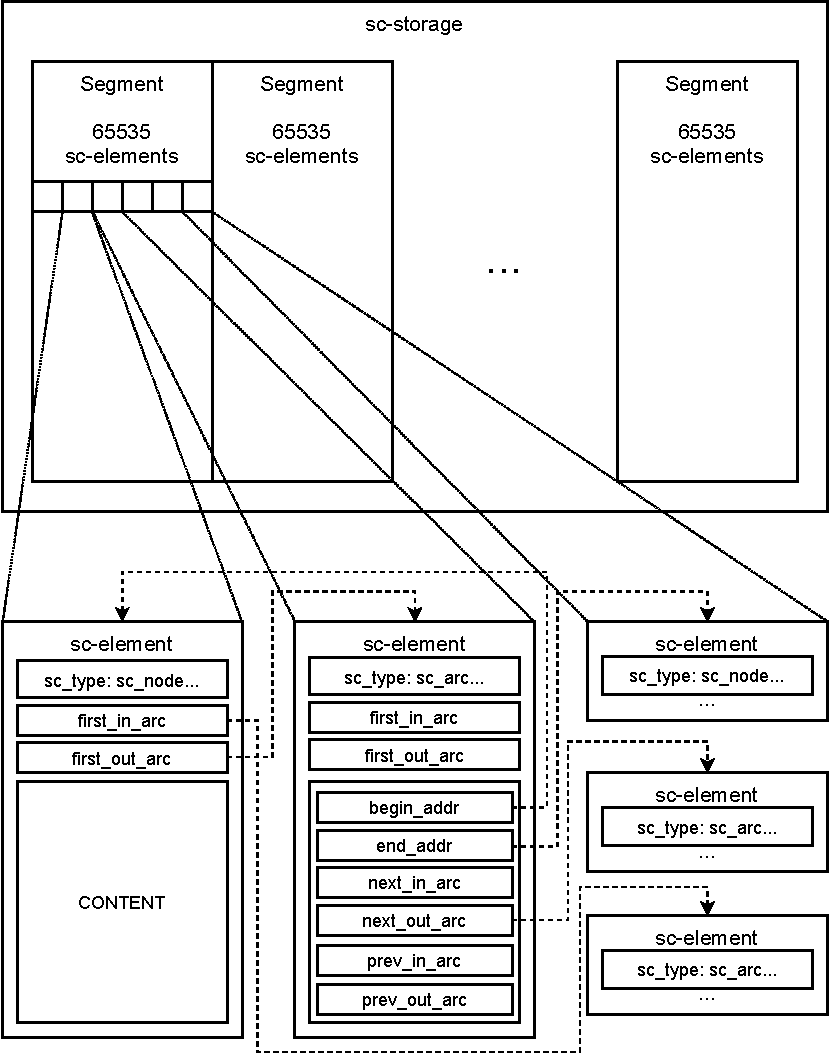
\includegraphics{images/sc_storage}}}
\scnrelfrom{класс объектов программной системы}{сегмент sc-хранилища}
\scnaddlevel{1}
\scnidtf{страница sc-хранилища}
\scnexplanation{В рамках данной реализации \textit{sc-хранилища} \scnbigspace \textit{sc-память} моделируется в виде набора \textit{сегментов}, каждый из которых представляет собой фиксированного размера упорядоченную последовательность \textit{элементов sc-хранилища}, каждый из которых соответствует конкретному sc-элементу. В настоящее время каждый сегмент состоит из $2^{16}-1=65535$ \textit{элементов sc-хранилища}. Выделение \textit{сегментов sc-хранилища} позволяет, с одной стороны, упростить адресный доступ к \textit{элементам sc-хранилища}, с другой стороны -- реализовать возможность выгрузки части sc-памяти из оперативной памяти на файловую систему при необходимости. Во втором случае сегмент sc-хранилища становится минимальной (атомарной) выгружаемой частью sc-памяти. Механизм выгрузки сегментов реализуется в соответствии с существующими принципами организации виртуальной памяти в современных операционных системах.}
\scnnote{Максимально возможное число сегментов ограничивается настройками программной реализации sc-хранилища (в настоящее время по умолчанию установлено количество $2^{16}-1=65535$ сегментов, но в общем случае оно может быть другим). Таким образом, технически максимальное количество хранимых sc-элементов в текущей реализации составляет около $4.3 \times 10^{9}$ sc-элементов.}
\scnnote{По умолчанию все сегменты физически располагаются в оперативной памяти, если объема памяти не хватает, то предусмотрен механизм выгрузки части сегментов на жесткий диск (механизм виртуальной памяти).}
\scnrelfrom{класс объектов программной системы}{элемент sc-хранилища}
\scnaddlevel{1}
\scnexplanation{Каждый сегмент состоит из набора структур данных, описывающих конкретные \textit{sc-элементы} (элементов sc-хранилища). Независимо от типа описываемого sc-элемента каждый \textit{элемент sc-хранилища} имеет фиксированный размер (в текущий момент -- 48 байт), что обеспечивает удобство их хранения. Таким образом, максимальный размер базы знаний в текущей программной модели sc-памяти может достигнуть 223 Гб (без учета содержимого \textit{внутренних файлов ostis-системы}, хранимого на внешней файловой системе).}
\scnaddlevel{-1}
\scnaddlevel{-1}
\scnrelfrom{пример}{\scnfilescg{images/sc_storage_example.png}}
\scnaddlevel{1}
\scnexplanation{Для наглядности в данном примере опущены \textit{метки уровня доступа}}
\scnaddlevel{-1}

\scnheader{sc-адрес}
\scnidtf{адрес элемента sc-хранилища, соответствующего заданному sc-элементу, в рамках текущего состояния реализации sc-хранилища в составе программной модели sc-памяти}
\scnexplanation{Каждый элемент sc-хранилища в текущей реализации может быть однозначно задан его адресом (sc-адресом), состоящим из номера сегмента и номера \textit{элемента sc-хранилища} в рамках сегмента. Таким образом, \textit{sc-адрес} служит уникальными координатами \textit{элемента sc-хранилища} в рамках \textit{Реализации sc-хранилища}.}
\scnnote{Sc-адрес никак не учитывается при обработке базы знаний на семантическом уровне и необходим только для обеспечения доступа к соответствующей структуре данных, хранящейся в линейной памяти на уровне \textit{Реализации sc-хранилища}.}
\scnnote{В общем случае sc-адрес элемента sc-хранилища, соответствующего заданному sc-элементу, может меняться, например, при пересборке базы знаний из исходных текстов и последующем перезапуске системы. При этом sc-адрес элемента sc-хранилища, соответствующего заданному sc-элементу, непосредственно в процессе работы системы в текущей реализации меняться не может.}
\scnnote{Для простоты будем говорить "sc-адрес sc-элемента"{}, имея в виду \textit{sc-адрес} \scnbigspace \textit{элемента sc-хранилища}, однозначно соответствующего данному \textit{sc-элементу}.}
\scnrelfromlist{семейство отношений, однозначно задающих структуру заданной сущности}{номер сегмента sc-хранилища*;номер элемента sc-хранилища в рамках сегмента*}

\scnheader{элемент sc-хранилища}
\scnidtf{ячейка sc-хранилища}
\scnidtf{элемент sc-хранилища, соответствующий sc-элементу}
\scnidtf{образ sc-элемента в рамках sc-хранилища}
\scnidtf{структура данных, каждый экземпляр которой соответствует одному sc-элементу в рамках sc-хранилища}
\scntext{пояснение}{Каждый элемент sc-хранилища, соответствующий некоторому sc-элементу, описывается его синтаксическим типом (меткой), а также независимо от типа указывается sc-адрес первой входящей в данный sc-элемент sc-дуги и первой выходящей из данного sc-элемента sc-дуги (могут быть пустыми, если таких sc-дуг нет).

Оставшиеся байты в зависимости от типа соответствующего sc-элемента (sc-узел или sc-дуга) могут использоваться либо для хранения содержимого внутреннего файла ostis-системы (может быть пустым, если sc-узел не является знаком файла), либо для хранения спецификации sc-дуги.}
\begin{scnrelfromset}{разбиение}
    \scnitem{элемент sc-хранилища, соответствующий sc-узлу}
    \begin{scnindent}
        \begin{scnrelfromset}{семейство отношений, однозначно задающих структуру заданной сущности}
            \scnitem{метка синтаксического типа sc-элемента*}
            \scnitem{метка уровня доступа sc-элемента*}
            \scnitem{sc-адрес первой sc-дуги, выходящей из данного sc-элемента*}
            \scnitem{sc-адрес первой sc-дуги, входящей в данный sc-элемент*}
            \scnitem{содержимое элемента sc-хранилища*}
            \begin{scnindent}
                \scnrelfrom{второй домен}{содержимое элемента sc-хранилища}
                \begin{scnindent}
                    \scnidtf{содержимое элемента sc-хранилища, соответствующего внутреннему файлу ostis-системы}
                \end{scnindent}
                \scntext{пояснение}{Каждый sc-узел в текущей реализации может иметь содержимое (может стать \textit{внутренним файлом ostis-системы}).
                В случае, если размер содержимого внутреннего файла ostis-системы не превышает 48 байт (размер \textit{спецификации sc-дуги в рамках sc-хранилища}, например небольшой \textit{строковый \mbox{sc-идентификатор}}), то это содержимое явно хранится в рамках элемента \mbox{sc-хранилища} в виде последовательности байт.
                В противном случае оно помещается в специальным образом организованную файловую память (за ее организацию отвечает отдельный модуль платформы, который в общем случае может быть устроен по-разному), а в рамках элемента sc-хранилища хранится уникальный адрес соответствующего файла, позволяющий быстро найти его на файловой системе.}
            \end{scnindent}
        \end{scnrelfromset}
        \begin{scnindent}
            \scntext{примечание}{\textit{sc-адрес первой sc-дуги, выходящей из данного sc-элемента*}, \textit{sc-адрес первой sc-дуги, входящей в данный sc-элемент*} и \textit{содержимое элемента sc-хранилища*} в общем случае могут отсутствовать (быть нулевыми, "пустыми"{}), но размер элемента в байтах останется тем же.}
        \end{scnindent}
    \end{scnindent}
    \scnitem{элемент sc-хранилища, соответствующий sc-дуге}
    \begin{scnindent}
        \begin{scnrelfromset}{семейство отношений, однозначно задающих структуру заданной сущности}
            \scnitem{метка синтаксического типа sc-элемента*}
            \scnitem{метка уровня доступа sc-элемента*}
            \scnitem{sc-адрес первой sc-дуги, выходящей из данного sc-элемента*}
            \scnitem{sc-адрес первой sc-дуги, входящей в данный sc-элемент*}
            \scnitem{спецификация sc-дуги в рамках sc-хранилища*}
            \begin{scnindent}
                \scnrelfrom{второй домен}{спецификация sc-дуги в рамках sc-хранилища}
                \begin{scnindent}
                    \begin{scnrelfromset}{семейство отношений, однозначно задающих структуру заданной сущности}
                        \scnitem{sc-адрес начального sc-элемента sc-дуги*}
                        \scnitem{sc-адрес конечного sc-элемента sc-дуги*}
                        \scnitem{sc-адрес следующей sc-дуги, выходящей из того же sc-элемента*}
                        \scnitem{sc-адрес следующей sc-дуги, входящей в тот же sc-элемент*}
                        \scnitem{sc-адрес предыдущей sc-дуги, выходящей из того же sc-элемента*}
                        \scnitem{sc-адрес предыдущей sc-дуги, входящей в тот же sc-элемент*}
                    \end{scnrelfromset}
                \end{scnindent}
            \end{scnindent}
        \end{scnrelfromset}
        \scntext{примечание}{sc-ребра в текущий момент хранятся так же, как sc-дуги, то есть имеют начальный и конечный sc-элементы, отличие заключается только в \textit{метке синтаксического типа sc-элемента}. Это приводит к ряду неудобств при обработке, но sc-ребра используются в настоящее время достаточно редко.}
    \end{scnindent}
\end{scnrelfromset}
\begin{scnindent}
    \scntext{примечание}{С точки зрения программной реализации структура данных для хранения sc-узла и sc-дуги остается остается та же, но в ней меняется список полей (компонентов).\\
    Кроме того, как можно заметить каждый элемент sc-хранилища (в том числе, \textit{элемент sc-хранилища, соответствующий sc-дуге}) не хранит список sc-адресов связанных с ним sc-элементов, а хранит sc-адреса одной выходящей и одной входящей дуги, каждая из которых в свою очередь хранит sc-адреса следующей и предыдущей дуг в списке исходящих и входящих sc-дуг для соответствующих элементов.
    Все перечисленное позволяет:
    \begin{scnitemize}
        \item сделать размер такой структуры фиксированным (в настоящее время 48 байт) и не зависящим от синтаксического типа хранимого sc-элемента;
        \item обеспечить возможность работы с sc-элементами без учета их синтаксического типа в случаях, когда это необходимо (например, при реализации поисковых запросов вида \scnqqi{Какие sc-элементы являются элементами данного множества}, \scnqqi{Какие sc-элементы непосредственно связаны с данным sc-элементом} и т.д.);
        \item обеспечить возможность доступа к \textit{элементу sc-хранилища} за константное время;
        \item обеспечить возможность помещения \textit{элемента sc-хранилища} в процессорный кэш, что в свою очередь, позволяет ускорить обработку sc-конструкций;
    \end{scnitemize}}
\end{scnindent}
\scntext{примечание}{Текущая \textit{Программная модель sc-памяти} предполагает, что вся sc-память физически расположена на одном компьютере. Для реализации распределенного варианта \textit{Программной модели sc-памяти} предполагается расширить \textit{sc-адрес} указанием адреса того физического устройства, где хранится соответствующий \textit{элемент sc-хранилища}.}

\scnheader{метка синтаксического типа sc-элемента}
\scnidtf{уникальный числовой идентификатор, однозначно соответствующий заданному типу sc-элементов и приписываемый соответствующему элементу sc-хранилища на уровне реализации}
\scntext{примечание}{Очевидно, что тип (класс, вид) sc-элемента в sc-памяти может быть задан путем явного указания принадлежности данного sc-элемента соответствующему классу (sc-узел, sc-дуга и т.д.).

Однако, в рамках \textit{платформы интерпретации sc-моделей компьютерных систем} должен существовать какой-либо набор \textit{меток синтаксического типа sc-элемента}, которые задают тип элемента на уровне платформы и не имеют соответствующей sc-дуги принадлежности (а точнее -- базовой sc-дуги), явно хранимой в рамках sc-памяти (ее наличие подразумевается, однако она не хранится явно, поскольку это приведет к бесконечному увеличению числа sc-элементов, которые необходимо хранить в sc-памяти). Как минимум, должна существовать метка, соответствующая классу \textit{базовая sc-дуга}, поскольку явное указание принадлежности sc-дуги данному классу порождает еще одну \textit{базовую sc-дугу}.

Таким образом, \textit{базовые sc-дуги}, обозначающие принадлежность sc-элементов некоторому известному ограниченному набору классов представлены неявно. Этот факт необходимо учитывать в ряде случаев, например, при проверке принадлежности sc-элемента некоторому классу, при поиске всех выходящих sc-дуг из заданного sc-элемента и т.д.

При необходимости некоторые из таких неявно хранимых sc-дуг могут быть представлены явно, например, в случае, когда такую sc-дугу необходимо включить в какое-либо множество, то есть провести в нее другую sc-дугу. В этом случае возникает необходимость синхронизации изменений, связанных с данной sc-дугой (например, ее удалении), в явном и неявном ее представлении. В текущей \textit{Реализации sc-хранилища} данный механизм не реализован.

Таким образом, полностью отказаться от \textit{меток синтаксического типа sc-элементов} невозможно, однако увеличение их числа хоть и повышает производительность платформы за счет упрощений некоторых операций по проверке типов sc-элемента, но приводит к увеличению числа ситуаций, в которых необходимо учитывать явное и неявное представление sc-дуг, что, в свою очередь, усложняет развитие платформы и разработку программного кода для обработки хранимых sc-конструкций.}
\scnrelto{второй домен}{метка синтаксического типа sc-элемента*}
\scnsuperset{метка sc-узла}
\begin{scnindent}
\scntext{числовое выражение в шестнадцатеричной системе}{0x1}
\end{scnindent}
\scnsuperset{метка внутреннего файла ostis-системы}
\begin{scnindent}
\scntext{числовое выражение в шестнадцатеричной системе}{0x2}
\end{scnindent}
\scnsuperset{метка sc-ребра общего вида}
\begin{scnindent}
\scntext{числовое выражение в шестнадцатеричной системе}{0x4}
\end{scnindent}
\scnsuperset{метка sc-дуги общего вида}
\begin{scnindent}
\scntext{числовое выражение в шестнадцатеричной системе}{0x8}
\end{scnindent}
\scnsuperset{метка sc-дуги принадлежности}
\begin{scnindent}
\scntext{числовое выражение в шестнадцатеричной системе}{0x10}
\end{scnindent}
\scnsuperset{метка sc-константы}
\begin{scnindent}
\scntext{числовое выражение в шестнадцатеричной системе}{0x20}
\end{scnindent}
\scnsuperset{метка sc-переменной}
\begin{scnindent}
\scntext{числовое выражение в шестнадцатеричной системе}{0x40}
\end{scnindent}
\scnsuperset{метка позитивной sc-дуги принадлежности}
\begin{scnindent}
\scntext{числовое выражение в шестнадцатеричной системе}{0x80}
\end{scnindent}
\scnsuperset{метка негативной sc-дуги принадлежности}
\begin{scnindent}
\scntext{числовое выражение в шестнадцатеричной системе}{0x100}
\end{scnindent}
\scnsuperset{метка нечеткой sc-дуги принадлежности}
\begin{scnindent}
\scntext{числовое выражение в шестнадцатеричной системе}{0x200}
\end{scnindent}
\scnsuperset{метка постоянной sc-дуги}
\begin{scnindent}
\scntext{числовое выражение в шестнадцатеричной системе}{0x400}
\end{scnindent}
\scnsuperset{метка временной sc-дуги}
\begin{scnindent}
\scntext{числовое выражение в шестнадцатеричной системе}{0x800}
\end{scnindent}
\scnsuperset{метка небинарной sc-связки}
\begin{scnindent}
\scntext{числовое выражение в шестнадцатеричной системе}{0x80}
\end{scnindent}
\scnsuperset{метка sc-структуры}
\begin{scnindent}
\scntext{числовое выражение в шестнадцатеричной системе}{0x100}
\end{scnindent}
\scnsuperset{метка ролевого отношения}
\begin{scnindent}
\scntext{числовое выражение в шестнадцатеричной системе}{0x200}
\end{scnindent}
\scnsuperset{метка неролевого отношения}
\begin{scnindent}
\scntext{числовое выражение в шестнадцатеричной системе}{0x400}
\end{scnindent}
\scnsuperset{метка sc-класса}
\begin{scnindent}
\scntext{числовое выражение в шестнадцатеричной системе}{0x800}
\end{scnindent}
\scnsuperset{метка абстрактной сущности}
\begin{scnindent}
\scntext{числовое выражение в шестнадцатеричной системе}{0x1000}
\end{scnindent}
\scnsuperset{метка материальной сущности}
\begin{scnindent}
\scntext{числовое выражение в шестнадцатеричной системе}{0x2000}
\end{scnindent}
\scnsuperset{метка константной позитивной постоянной sc-дуги принадлежности}
\begin{scnindent}
\scnidtf{метка базовой sc-дуги}
\scnidtf{метка sc-дуги основного вида}
\begin{scnreltoset}{пересечение}
    \scnitem{метка sc-дуги принадлежности}
    \scnitem{метка sc-константы;метка позитивной sc-дуги принадлежности}
    \scnitem{метка постоянной sc-дуги}
\end{scnreltoset}
\scntext{примечание}{\textit{метки синтаксических типов sc-элементов} могут комбинироваться между собой для получения более частных классов меток. С точки зрения программной реализации такая комбинация выражается операцией побитового сложения значений соответствующих меток.}
\end{scnindent}
\scnsuperset{метка переменной позитивной постоянной sc-дуги принадлежности}
\begin{scnindent}
\begin{scnreltoset}{пересечение}
    \scnitem{метка sc-дуги принадлежности}
    \scnitem{метка sc-переменной}
    \scnitem{метка позитивной sc-дуги принадлежности;метка постоянной sc-дуги}
\end{scnreltoset}
\end{scnindent}
\scntext{примечание}{Числовые выражения некоторых классов меток могут совпадать. Это сделано для уменьшения размера элемента sc-хранилища за счет уменьшения максимального размера метки. Конфликт в данном случае не возникает, поскольку такие классы меток не могут комбинироваться, например \textit{метка ролевого отношения} и \textit{метка нечеткой sc-дуги принадлежности}.}
\scntext{примечание}{Важно отметить, что каждому из выделенных классов меток (кроме классов, получаемых путем комбинации других классов) однозначно соответствует порядковый номер бита в линейной памяти, что можно заметить, глядя на соответствующие числовые выражения классов меток. Это означает, что классы меток не включаются друг в друга, например, указание \textit{метки позитивной sc-дуги принадлежности} не означает автоматическое указание \textit{метки sc-дуги принадлежности}. Это позволяет сделать операции комбинирования и сравнения меток более эффективными.}
\begin{scnreltoset}{недостатки текущего состояния}
    \scnitem{\scnfilelong{На данный момент число \textit{меток синтаксического типа sc-элемента} достаточно велико, что приводит к возникновению достаточно большого числа ситуаций, в которых нужно учитывать явное и неявное хранение sc-дуг принадлежности соответствующим классам. С другой стороны, изменение набора меток с какой-либо целью в текущем варианте реализации представляет собой достаточно трудоемкую задачу (с точки зрения объема изменений в программном коде платформы и sc-агентов, реализованных на уровне платформы), а расширение набора меток без увеличения объема элемента sc-хранилища в байтах оказывается и вовсе невозможным.}}
    \begin{scnindent}
        \scntext{вариант решения}{Решением данной проблемы является максимально возможная минимизация числа меток, например, до числа меток, соответствующих \textit{Алфавиту SC-кода}. В таком случае принадлежность sc-элементов любым другим классам будет записываться явно, а число ситуаций, в которых необходимо будет учитывать неявное хранение sc-дуг, будет минимальным.}
    \end{scnindent}
    \scnitem{\scnfilelong{Некоторые метки из текущего набора \textit{меток синтаксического типа sc-элемента} используются достаточно редко (например, \textit{метка sc-ребра общего вида} или \textit{метка негативной sc-дуги принадлежности}), в свою очередь, в sc-памяти могут существовать классы, имеющие достаточно много элементов (например, \textit{бинарное отношение} или \textit{число}). Данный факт не позволяет в полной мере использовать эффективность наличия меток.}}
    \begin{scnindent}
        \scntext{вариант решения}{Решением данной проблемы является отказ от заранее известного набора меток и переход к динамическому набору меток (при этом их число может оставаться фиксированным). В этом случае набор классов, выражаемых в виде меток будет формироваться на основании каких-либо критериев, например, числа элементов данного класса или частоты обращений к нему.}
    \end{scnindent}
\end{scnreltoset}

\scnheader{метка уровня доступа sc-элемента}
\scnrelto{второй домен}{метка уровня доступа sc-элемента*}
\scnrelfromset{обобщенная структура}{метка уровня доступа sc-элемента на чтение;метка уровня доступа sc-элемента на запись}
\scnexplanation{В текущей \textit{Реализации sc-хранилища} \scnbigspace \textit{метки уровня доступа} используются для того, чтобы обеспечить возможность ограничения доутспа некоторых процессов в sc-памяти к некоторым sc-элементам, хранимым в sc-памяти.

Каждому элементу sc-хранилища соответствует \textit{метка уровня доступа sc-элемента на чтение} и \textit{метка уровня доступа sc-элемента на запись}, каждая из которых выражается числом от 0 до 255.

В свою очередь, каждому процессу (чаще всего, соответствующему некоторому sc-агенту), который пытается получить доступ к данному элементу sc-хранилища (прочитать или изменить его) соответствует уровень доступа на чтение и запись, выраженный в том же числовом диапазоне. Указанный уровень доступа для процесса является частью \textit{контекста процесса}. Доступ на чтение или запись к элементу sc-хранилища не разрешается, если уровень доступа соответственно на чтение или запись у процесса ниже, чем у элемента sc-хранилища, к которому осуществляется доступ.

Таким образом нулевое значение \textit{метки уровня доступа sc-элемента на чтение} и \textit{метки уровня доступа sc-элемента на запись} означает, что любой процесс может получить неограниченный доступ к данному элементу sc-хранилища.}

